\documentclass[conference,letterpaper]{IEEEtran}
\IEEEoverridecommandlockouts
% Toque MCIC sobre IEEEtran: solo color y diagramas. No cambia márgenes,
% fuentes, columnas ni tamaños de la plantilla IEEE.
% tectonic compila con XeTeX: Times New Roman (la de IEEE y la secundaria del manual UD)
% se lee de las fuentes del manual de marca; si no está, TeX Gyre Termes (clon de Times).
\usepackage{amsmath,amssymb}
\usepackage{newtxmath}
\usepackage{fontspec}
\providecommand{\UDmarca}{/Users/juferoga/repos/ud/maestria/mcic/.UniversidadDistrital-manual-marca}
\IfFileExists{\UDmarca/fuentes/times.ttf}{%
  \setmainfont{times.ttf}[Path=\UDmarca/fuentes/, BoldFont=timesbd.ttf,
    ItalicFont=timesi.ttf, BoldItalicFont=timesbi.ttf]}{%
  \setmainfont{texgyretermes}[Extension=.otf, UprightFont=*-regular, BoldFont=*-bold,
    ItalicFont=*-italic, BoldItalicFont=*-bolditalic]}
\setmonofont{texgyrecursor}[Extension=.otf, UprightFont=*-regular, BoldFont=*-bold, Scale=0.95]
\usepackage[spanish,es-noshorthands,es-tabla,es-nolists]{babel}
\usepackage{graphicx}
\usepackage{booktabs,tabularx,array,multirow}
\usepackage[table]{xcolor}
\usepackage{tikz}
\usetikzlibrary{positioning,arrows.meta,calc,fit}
\usepackage[hidelinks]{hyperref}
\usepackage{cite}
\usepackage{url}

% Paleta del manual de marca UD (design.md)
\definecolor{udazul}{HTML}{1291C0}
\definecolor{udazulosc}{HTML}{0C6F96}
\definecolor{uddorado}{HTML}{B49739}
\definecolor{udverde}{HTML}{00A859}
\definecolor{udplata}{HTML}{98999A}
\definecolor{udsable}{HTML}{373435}
\definecolor{udrojo}{HTML}{ED3237}

\hypersetup{colorlinks=true,linkcolor=udazulosc,citecolor=udazulosc,urlcolor=udazulosc}

% Bloques de la ecuación de búsqueda: el mismo color en ecuación, PRISMA y matriz.
\newcommand{\bloqueA}[1]{\textcolor{udazulosc}{#1}}
\newcommand{\bloqueB}[1]{\textcolor{uddorado!85!black}{#1}}
\newcommand{\bloqueC}[1]{\textcolor{udverde!80!black}{#1}}
\newcommand{\etiqueta}[2]{\tikz[baseline=(t.base)]\node[fill=#1,text=white,inner sep=1.6pt,
  rounded corners=1pt,font=\bfseries\scriptsize](t){#2};}

% Cabecera de tablas: filete azul y fila sombreada clara
\newcommand{\cabecera}{\rowcolor{udazul!12}}
\arrayrulecolor{udazulosc}

% Columnas de la matriz
\newcolumntype{L}[1]{>{\raggedright\arraybackslash}p{#1}}
\newcolumntype{Y}{>{\raggedright\arraybackslash}X}

\makeatletter
\providecommand{\filas}[1]{\@@input #1 }
\makeatother

% Marca de enfoque en la matriz (A..E)
\newcommand{\enf}[1]{\textcolor{udazulosc}{\bfseries #1}}

% Cajas del PRISMA
\tikzset{
  caja/.style={draw=udazulosc,line width=0.5pt,rounded corners=1.5pt,align=center,
    font=\scriptsize,inner sep=2.5pt,text width=#1},
  caja/.default=3.6cm,
  excl/.style={draw=udplata,line width=0.5pt,rounded corners=1.5pt,align=left,
    font=\scriptsize,inner sep=2.5pt,fill=udplata!8,text width=#1},
  excl/.default=2.75cm,
  fase/.style={fill=udazul,text=white,font=\bfseries\tiny,minimum width=0.42cm,
    rounded corners=1pt,inner sep=1pt},
  flecha/.style={-{Latex[length=1.6mm]},udsable,line width=0.5pt},
}

% Generado por revision/generar_e1.py; no editar a mano.
\newcommand{\nArxivQuno}{35}
\newcommand{\nArxivQdos}{3}
\newcommand{\nArxivTotal}{38}
\newcommand{\nArxivDup}{0}
\newcommand{\nOaQuno}{162}
\newcommand{\nOaQdos}{33}
\newcommand{\nOaTotal}{195}
\newcommand{\nOaDup}{39}
\newcommand{\nDup}{39}
\newcommand{\nTamizados}{194}
\newcommand{\nExclTitulo}{147}
\newcommand{\nPasan}{47}
\newcommand{\nExclTexto}{10}
\newcommand{\nIncluidosBases}{37}
\newcommand{\nOtros}{21}
\newcommand{\nTotalIncluidos}{58}
\newcommand{\nMatriz}{16}
\newcommand{\nMatrizRecientes}{13}
\newcommand{\nRecientes}{49}
\newcommand{\nTextoCompleto}{35}
\newcommand{\nSoloResumen}{23}
\newcommand{\fechaConsulta}{2026-11-06}
\newcommand{\fechaConsultaOa}{2026-11-07}

% Generado por articulo/generar_cifras.py; no editar a mano.
\newcommand{\cifCommits}{612.811}
\newcommand{\cifDesarrollo}{558.438}
\newcommand{\cifPrueba}{54.373}
\newcommand{\cifPrevMin}{3{,}9\,\%}
\newcommand{\cifPrevMax}{4{,}5\,\%}
\newcommand{\cifPrevAnioVeintiseis}{3{,}39\,\%}
\newcommand{\cifPositivosDesarrollo}{23.735}
\newcommand{\cifPositivosPrueba}{1.947}
\newcommand{\cifCensurados}{26.133}
\newcommand{\cifAutores}{18.127}
\newcommand{\cifSubsistemas}{748}
\newcommand{\cifNVariables}{22}
\newcommand{\cifPrevQunoAdd}{0{,}9\,\%}
\newcommand{\cifPrevQcincoAdd}{11{,}7\,\%}
\newcommand{\cifReviewedIni}{0{,}42}
\newcommand{\cifReviewedFin}{0{,}71}
\newcommand{\cifFixIni}{14{,}5\,\%}
\newcommand{\cifFixFin}{18{,}4\,\%}
\newcommand{\cifValMayoritaria}{0{,}0410}
\newcommand{\cifValLogistica}{0{,}1486}
\newcommand{\cifValGB}{0{,}1578}
\newcommand{\cifParamGB}{5.645}
\newcommand{\cifParamLR}{23}
\newcommand{\cifNConfigsRef}{10}
\newcommand{\cifValFE}{0{,}1495}
\newcommand{\cifValFEde}{0{,}0053}
\newcommand{\cifValVariante}{0{,}1206}
\newcommand{\cifReglasMin}{3}
\newcommand{\cifReglasMax}{6}
\newcommand{\cifAntMin}{3}
\newcommand{\cifAntMax}{10}
\newcommand{\cifTiempoFE}{11}
\newcommand{\cifNBusqueda}{14}
\newcommand{\cifMejorBusqueda}{0{,}1485}
\newcommand{\cifRazonValFE}{94{,}8\,\%}
\newcommand{\cifCongelada}{2026-11-07 23:41}
\newcommand{\cifHuella}{11e7039f3cc27912}
\newcommand{\cifSemillaRef}{11}
\newcommand{\cifSensMax}{0{,}1498}
\newcommand{\cifSensMaxR}{10}
\newcommand{\cifSensMaxPm}{0{,}05}
\newcommand{\cifSensMin}{0{,}1305}
\newcommand{\cifSensMinR}{15}
\newcommand{\cifSensMinPm}{0{,}30}
\newcommand{\cifSensMutBaja}{0{,}1486}
\newcommand{\cifSensMutAlta}{0{,}1347}
\newcommand{\cifReglasVariante}{15}
\newcommand{\cifAntVariante}{29}
\newcommand{\cifRegReferencias}{30}
\newcommand{\cifRegPropuesto}{84}
\newcommand{\cifRegBusq}{42}
\newcommand{\cifRegSens}{24}
\newcommand{\cifTestMay}{0{,}0346}
\newcommand{\cifTestMayde}{0{,}0000}
\newcommand{\cifTestMayic}{[0{,}033;\ 0{,}036]}
\newcommand{\cifCaidaMay}{15{,}5\,\%}
\newcommand{\cifTestLR}{0{,}1274}
\newcommand{\cifTestLRde}{0{,}0000}
\newcommand{\cifTestLRic}{[0{,}117;\ 0{,}140]}
\newcommand{\cifCaidaLR}{14{,}2\,\%}
\newcommand{\cifTestGB}{0{,}1320}
\newcommand{\cifTestGBde}{0{,}0007}
\newcommand{\cifTestGBic}{[0{,}121;\ 0{,}146]}
\newcommand{\cifCaidaGB}{16{,}3\,\%}
\newcommand{\cifTestVar}{0{,}0901}
\newcommand{\cifTestVarde}{0{,}0000}
\newcommand{\cifTestVaric}{[0{,}083;\ 0{,}098]}
\newcommand{\cifCaidaVar}{25{,}3\,\%}
\newcommand{\cifTestFE}{0{,}1202}
\newcommand{\cifTestFEde}{0{,}0024}
\newcommand{\cifTestFEic}{[0{,}108;\ 0{,}128]}
\newcommand{\cifCaidaFE}{19{,}5\,\%}
\newcommand{\cifPrevPrueba}{3{,}46\,\%}
\newcommand{\cifNPrueba}{54.373}
\newcommand{\cifCuno}{91{,}1\,\%}
\newcommand{\cifFriedmanP}{0{,}0043}
\newcommand{\cifNemenyiCD}{3{,}05}
\newcommand{\cifAssistedN}{2.031}
\newcommand{\cifAssistedPrev}{2{,}81\,\%}
\newcommand{\cifAssistedLR}{0{,}079}
\newcommand{\cifSinAssistedLR}{0{,}130}
\newcommand{\cifAssistedGB}{0{,}067}
\newcommand{\cifSinAssistedGB}{0{,}136}
\newcommand{\cifAssistedFE}{0{,}055}
\newcommand{\cifSinAssistedFE}{0{,}120}
\newcommand{\cifFEMarcMin}{0{,}0\,\%}
\newcommand{\cifFEMarcMax}{17{,}9\,\%}
\newcommand{\cifFEMccMin}{0{,}000}
\newcommand{\cifFEMccMax}{0{,}175}
\newcommand{\cifFEApMin}{0{,}1172}
\newcommand{\cifFEApMax}{0{,}1245}
\newcommand{\cifFERefMarc}{17{,}9\,\%}
\newcommand{\cifFERefAp}{0{,}1172}
\newcommand{\cifMcAciertaGB}{584}
\newcommand{\cifMcFallaGB}{4.379}
\newcommand{\cifMcAciertaLR}{667}
\newcommand{\cifMcFallaLR}{3.422}
\newcommand{\cifMcAciertaVar}{3.306}
\newcommand{\cifMcFallaVar}{878}
\newcommand{\cifNReglasRef}{5}
\newcommand{\cifParamFE}{27}
\newcommand{\cifParamGBprueba}{5.765}
\newcommand{\cifErrQcincoSens}{86{,}8\,\%}
\newcommand{\cifErrQcincoPrev}{9{,}6\,\%}
\newcommand{\cifErrQunoPrev}{0{,}8\,\%}
\newcommand{\cifErrFixAp}{0{,}088}
\newcommand{\cifErrNoFixAp}{0{,}126}
\newcommand{\cifErrFixSens}{20{,}3\,\%}
\newcommand{\cifErrNoFixSens}{58{,}7\,\%}
\newcommand{\cifMesIni}{0{,}151}
\newcommand{\cifMesFin}{0{,}086}
\newcommand{\cifMesGBIni}{0{,}158}
\newcommand{\cifMesGBFin}{0{,}104}
\newcommand{\cifRangoFE}{2{,}50}
\newcommand{\cifRangoGB}{1{,}00}
\newcommand{\cifRangoLR}{2{,}50}
\newcommand{\cifRangoVar}{4{,}00}
\newcommand{\cifRangoMay}{5{,}00}
\newcommand{\cifAporteEvolPrueba}{33\,\%}
\newcommand{\cifItDosCreOriFE}{0{,}1485}
\newcommand{\cifItDosCreOriGB}{0{,}1578}
\newcommand{\cifItDosCreOriRazon}{0{,}941}
\newcommand{\cifItDosCreAmpFE}{0{,}1472}
\newcommand{\cifItDosCreAmpGB}{0{,}1578}
\newcommand{\cifItDosCreAmpRazon}{0{,}933}
\newcommand{\cifItDosDesOriFE}{0{,}1478}
\newcommand{\cifItDosDesOriGB}{0{,}1577}
\newcommand{\cifItDosDesOriRazon}{0{,}937}
\newcommand{\cifItDosDesAmpFE}{0{,}1428}
\newcommand{\cifItDosDesAmpGB}{0{,}1577}
\newcommand{\cifItDosDesAmpRazon}{0{,}905}
\newcommand{\cifItDosUmbral}{0{,}947}
\newcommand{\cifItDosAdoptada}{no}

\renewcommand{\IEEEkeywordsname}{Palabras clave}
\newcommand{\pendiente}[1]{\textcolor{udrojo}{\textbf{[#1]}}}
\raggedbottom

\begin{document}

\title{Riesgo de los commits del kernel de Linux bajo deriva temporal: un clasificador difuso-evolutivo interpretable: estado del arte, datos, modelos, evaluación y experimentación}

\author{\IEEEauthorblockN{Juan Felipe Rodríguez Galindo}
\IEEEauthorblockA{Maestría en Ciencias de la Información y las Comunicaciones\\
Universidad Distrital Francisco José de Caldas, Bogotá, Colombia\\
Código 20261595004 \textperiodcentered{} Inteligencia Computacional \textperiodcentered{} Entregable 4}}

\maketitle

\begin{abstract}
Predecir si un commit tendrá que corregirse después permite enfocar la revisión de código. En el kernel de Linux la etiqueta es explícita: el trailer \texttt{Fixes:} de un commit posterior señala al culpable. Se plantean el problema, la pregunta y el criterio de éxito del proyecto, y se presenta una revisión estructurada tipo PRISMA en arXiv y OpenAlex con \nTotalIncluidos{} estudios incluidos (37 citados aquí; la matriz completa va en el anexo, \nRecientes{} desde 2021). La predicción justo a tiempo (JIT) se valida casi siempre con un único corte o con validación cruzada aleatoria y se mide con AUC-ROC, F1 o exactitud. A nivel de commit, lo difuso y lo evolutivo solo aparecen como piezas auxiliares (agrupamiento o ajuste de parámetros); como clasificador, solo a nivel de módulo. Se construye además el dataset: \cifCommits{} commits de 2019--2026 minados del clon completo del kernel, con prevalencia de \cifPrevMin{}--\cifPrevMax{}, se justifican los cinco modelos que se comparan y se declara el protocolo de evaluación: partición temporal con hueco de 90 días, AUC-PR como métrica principal, McNemar y Friedman--Nemenyi. En validación, el \emph{gradient boosting} alcanza un AUC-PR de \cifValGB{} y la regresión logística \cifValLogistica{}, frente a una prevalencia de \cifValMayoritaria{}. Tras una búsqueda aleatoria, un análisis de sensibilidad y 5 semillas, el modelo propuesto llega a \cifValFE{} $\pm$ \cifValFEde{} con solo \cifReglasMin{}--\cifReglasMax{} reglas, y la evolución aporta frente a la variante sin evolución (\cifValVariante{}). Ningún trabajo evalúa un clasificador de reglas difusas a nivel de commit con validación temporal y AUC-PR, ni su degradación en 2026, el año en que el kernel pidió y luego retiró la etiqueta \texttt{Assisted-by} para contribuciones asistidas por IA.
\end{abstract}

\begingroup\renewcommand{\abstractname}{Abstract}
\begin{abstract}
We frame a project on just-in-time risk prediction for Linux kernel commits, labelled by later \texttt{Fixes:} trailers, and report a PRISMA-style review (arXiv and OpenAlex, \nTotalIncluidos{} included studies, 37 cited here; the full matrix is in the appendix). No prior work evaluates an evolutionarily tuned fuzzy rule classifier at commit level with temporal validation and AUC-PR, nor its degradation on 2026 commits.
\end{abstract}\endgroup

\begin{IEEEkeywords}
predicción de defectos justo a tiempo, kernel de Linux, deriva temporal, sistemas difusos, computación evolutiva, AUC-PR.
\end{IEEEkeywords}

%=====================================================================
\section{Introducción}

Desde hace dos décadas, el riesgo de un commit se estima con métricas del propio cambio: cuánto toca, cuánto se difunde y la experiencia del autor \cite{Mockus2000,Kamei2013}. Es la predicción justo a tiempo (JIT): la alerta llega cuando el cambio aún está en revisión. El kernel de Linux cuenta con una ventaja clave: cuando un commit corrige un fallo previo, el trailer \texttt{Fixes:} identifica explícitamente al culpable sin recurrir a heurísticas como SZZ mediante \texttt{git blame} \cite{Sliwerski2005}. En estudios empíricos, el 81\,\% se confirmó como causa del bug; el resto es ambiguo o incorrecto \cite{Lyu2024}.

En 2026 cambió quién escribe parte de estos cambios. La versión 7.0 pidió declarar con \texttt{Assisted-by:} la ayuda de asistentes de IA \cite{KernelAdd}, simplificada luego a \texttt{Assisted-by: LLM} \cite{KernelSimpl}. El 14 de octubre se retiró al constatar que solo cerca del 10\,\% de los commits la incluía, pese a un uso real mucho mayor \cite{KernelRemove}. Por ello, la <<era de la IA>> se define por frontera temporal (Fig.~\ref{fig:tiempo}) y no por la etiqueta, que queda solo como referencia complementaria.

\begin{figure}[!t]
\centering
% Fig. 1: ventanas de datos frente a los hitos del trailer Assisted-by.
% Eje izquierdo esquemático (2019-2025); 2026 a escala por meses (0,58 cm por mes).
\begin{tikzpicture}[x=1cm,y=1cm,font=\scriptsize]
  \def\m{0.5}           % ancho de un mes de 2026
  \def\xo{2.6}          % inicio de 2026 en el eje
  % --- bandas de datos
  \fill[udazul!18] (0,0) rectangle (\xo,0.42);
  \node[udazulosc,align=center,font=\tiny\bfseries] at (\xo/2,0.21) {entrenamiento y validación\\ móvil (2019--2025)};
  \fill[uddorado!30] (\xo,0) rectangle ({\xo+7*\m},0.42);
  \node[uddorado!60!black,font=\tiny\bfseries] at ({\xo+3.5*\m},0.21) {prueba: ene--jul 2026};
  \fill[udplata!25] ({\xo+7*\m},0) rectangle ({\xo+10.2*\m},0.42);
  \node[udsable,align=center,font=\tiny] at ({\xo+8.6*\m},0.21) {censura\\ ($<$90 d)};
  % --- eje
  \draw[udsable,line width=0.5pt] (0,0) -- ({\xo+10.4*\m},0);
  \draw[udsable,line width=0.5pt] (\xo-0.42,-0.08) -- (\xo-0.34,0.08);
  \draw[udsable,line width=0.5pt] (\xo-0.34,-0.08) -- (\xo-0.26,0.08);
  \foreach \x/\t in {0/2019, 1.9/2025} \node[below,udsable] at (\x,0) {\t};
  \foreach \i/\t in {0/ene,2/mar,4/may,6/jul,8/sep,10/nov}
    {\draw[udsable] ({\xo+\i*\m},0) -- ++(0,-0.06);
     \node[below,udsable] at ({\xo+\i*\m},-0.02) {\t};}
  \node[below=7pt,udsable,font=\tiny\bfseries] at ({\xo+5*\m},0) {2026};
  % --- hitos del trailer (encima del eje)
  \foreach \x/\t/\yy in {0.17/v7.0: se pide \texttt{Assisted-by}/0.95,
                          7.07/v7.3: solo ``\texttt{LLM}''/1.35,
                          9.45/v7.4: se elimina/0.95}{
    \draw[udrojo,line width=0.6pt] ({\xo+\x*\m},0.42) -- ({\xo+\x*\m},\yy-0.08);
    \fill[udrojo] ({\xo+\x*\m},\yy-0.08) circle (1.1pt);
    \node[udrojo,above,font=\tiny,inner sep=1pt] at ({\xo+\x*\m},\yy-0.06) {\t};}
  % --- corte de observación
  \draw[udsable,dashed] ({\xo+10.2*\m},-0.05) -- ({\xo+10.2*\m},0.6)
     node[above,font=\tiny,udsable,inner sep=1pt] {corte};
\end{tikzpicture}

\caption{Diseño temporal propuesto frente a los hitos de \texttt{Assisted-by} \cite{KernelAdd,KernelSimpl,KernelRemove}. Los commits posteriores a julio de 2026 quedan censurados: no han tenido los 90 días para recibir un \texttt{Fixes:}.}
\label{fig:tiempo}
\end{figure}

\subsection{Problema y pregunta de investigación}

\textbf{Problema.} Clasificar cada commit del kernel como \emph{riesgoso} si un commit posterior lo cita con \texttt{Fixes:} en 90 días o menos, usando solo información disponible en el momento de integrarlo, y con un modelo que un mantenedor pueda leer.

\textbf{Pregunta.} ¿Un clasificador de a lo sumo 15 reglas difusas, cuyas funciones de pertenencia y reglas se ajustan con un algoritmo evolutivo, alcanza en los commits de 2026 un AUC-PR de al menos el 90\,\% del mejor modelo de referencia (regresión logística o \emph{gradient boosting}), y pierde menos AUC-PR que ese modelo al pasar de la validación (ventanas anuales 2023, 2024 y 2025, entrenando desde 2019) a la prueba (enero--julio de 2026)?

\subsection{Criterio de éxito (etapa 1 de CRISP-ML(Q) \cite{Studer2021})}

Sea $\mathrm{AP}_m^{V}$ el AUC-PR medio del modelo $m$ en las ventanas de validación y $\mathrm{AP}_m^{T}$ su AUC-PR en la prueba de 2026, ambos con intervalo de confianza del 95\,\% por \emph{bootstrap}. Sean $\Delta_m=(\mathrm{AP}_m^{V}-\mathrm{AP}_m^{T})/\mathrm{AP}_m^{V}$ la caída relativa, $\pi^{T}$ la prevalencia de positivos en la prueba (el AUC-PR de la clase mayoritaria), FE el modelo propuesto y $R$ la mejor referencia clásica en validación. El proyecto se declara exitoso si se cumplen las tres condiciones de la Tabla~\ref{tab:criterio}. Si no se cumplen, se reporta así, sin volver a ajustar nada con la prueba.

\begin{table}[!t]
\caption{Criterio de éxito, fijado antes de ver los datos}
\label{tab:criterio}
\centering\footnotesize
\begin{tabularx}{\columnwidth}{@{}l Y@{}}
\toprule
\cabecera & \textbf{Condición}\\
\midrule
C1 Desempeño & $\mathrm{AP}_{FE}^{T}\ge 0{,}90\,\mathrm{AP}_{R}^{T}$\\
C2 Robustez & $\Delta_{FE}<\Delta_{R}$ (diferencia observada, con IC 95\,\%)\\
C3 Piso & El IC 95\,\% de $\mathrm{AP}_{FE}^{T}$ excluye $\pi^{T}$; McNemar contra cada referencia con $\alpha=0{,}05$\\
Restricción & $\le$15 reglas y $\le$3 antecedentes por regla\\
\bottomrule
\end{tabularx}
\end{table}

\subsection{Datos y consideraciones éticas}
Los datos son públicos: el historial oficial de \texttt{torvalds/linux} (GPL-2.0), minado directamente para un registro continuo de 2014 a 2026. Para contrastar la etiqueta se recurre además al dataset de Maes Bermejo \emph{et al.} en Zenodo \cite{MaesBermejo2024}. Por ser fuentes enteramente abiertas no se requiere aprobación de un comité de ética; por privacidad, los nombres y correos de los autores se sustituyen por identificadores anónimos.


%=====================================================================
\section{Estado del arte}

\subsection{Método de búsqueda}
La búsqueda sigue las directrices de PRISMA 2020 \cite{Page2021} en versión sintetizada. El problema se descompone en tres componentes temáticos esenciales, unidos con OR por dentro y AND entre ellos:

\noindent\fbox{\parbox{\dimexpr\columnwidth-2\fboxsep-2\fboxrule}{\footnotesize\raggedright
\etiqueta{udazulosc}{A} \bloqueA{(commit* OR ``code change*'' OR ``software change*'' OR patch* OR ``pull request*'' OR ``Linux kernel'')} AND\\
\etiqueta{uddorado}{B} \bloqueB{(``defect prediction'' OR ``bug prediction'' OR ``bug-introducing'' OR ``bug-inducing'' OR ``fix-inducing'' OR ``just-in-time'' OR ``change risk'' OR ``risk prediction'' OR ``defect-prone'' OR buggy)} AND\\
\etiqueta{udverde}{C} \bloqueC{(fuzzy OR ``rule-based'' OR evolutionary OR ``genetic algorithm'' OR ``genetic programming'' OR ``search-based'' OR interpretab* OR explainab*)}}}

\smallskip
La ecuación Q1 combina los tres bloques. La Q2 cambia el bloque C por deriva temporal (``concept drift'', drift, ``temporal validation'', ``time-aware'', ``realistic evaluation'', ``data shift'', ``distribution shift'', ``time travel''). Ambas consultas se ejecutaron sobre 2019--2026 vía APIs públicas en arXiv y OpenAlex (título y resumen) para garantizar reproducibilidad. OpenAlex indexa IEEE, ACM, Springer y Elsevier, supliendo la falta de acceso institucional a Scopus o IEEE Xplore. Clásicos previos a 2019 o hallados por citas entran como ``otras fuentes''.

Los criterios se definieron antes del tamizaje. Se incluye si: (I1) predice el riesgo de un cambio o estudia la validez de esa evaluación (orden temporal, latencia, ruido), (I2) reporta métricas cuantitativas, y (I3) describe sus datos. Se excluye si: (E1) trata generación o reparación de código, (E2) evalúa solo a nivel de archivo o módulo (se admitieron propuestas difusas y evolutivas de módulo ante la ausencia a nivel de commit), (E3) es de otro dominio, (E4) es solo un dataset sin modelo, o (E5) no se puede verificar. De las bases se evaluaron \nPasan{} registros en elegibilidad (\nExclTexto{} excluidos y \nIncluidosBases{} incluidos); a estos se sumaron \nOtros{} de otras fuentes bajo los mismos criterios I y E, totalizando \nTotalIncluidos{} estudios incluidos (37 citados aquí; la matriz completa va en el anexo). De ellos, \nTextoCompleto{} se leyeron a texto completo y \nSoloResumen{} por resumen o fuentes secundarias debido a restricciones de acceso institucional. El flujo se resume en la Fig.~\ref{fig:prisma}.

\begin{figure}[!t]
\centering
% Fig. 2: diagrama de flujo tipo PRISMA 2020. Todos los números son macros de generado/conteos.tex.
\begin{tikzpicture}[node distance=2.6mm and 2.4mm]
  % Identificación
  \node[caja=3.75cm] (bases) {\textbf{Bases de datos} (2019--2026)\\
     arXiv: Q1 \nArxivQuno{} $+$ Q2 \nArxivQdos{} $=$ \nArxivTotal\\
     OpenAlex: Q1 \nOaQuno{} $+$ Q2 \nOaQdos{} $=$ \nOaTotal};
  \node[caja=2.45cm,right=of bases] (otros) {\textbf{Otras fuentes}\\ clásicos, citas y
     búsqueda dirigida: \nOtros};
  % Tamizaje
  \node[caja=3.75cm,below=4mm of bases] (tam) {\textbf{Tamizaje por título y resumen}\\
     \nTamizados{} registros (sin \nDup{} duplicados)};
  \node[excl,right=of tam] (extam) {Excluidos (E1--E5): \nExclTitulo};
  \node[caja=3.75cm,below=of tam] (tc) {\textbf{Evaluados en elegibilidad}: \nPasan};
  \node[excl,right=of tc] (extc) {Excluidos tras leer: \nExclTexto};
  \node[caja=3.75cm,below=of tc,fill=udazul!10] (inc) {\textbf{Incluidos: \nTotalIncluidos}
     (\nIncluidosBases{} de bases $+$ \nOtros{} de otras fuentes)\\ \nRecientes{} desde 2021;
     \nMatriz{} en la Tabla~\ref{tab:matriz}};
  \draw[flecha] (bases) -- (tam);
  \draw[flecha] (tam) -- (tc);
  \draw[flecha] (tc) -- (inc);
  \draw[flecha] (otros.east) -- ++(1.6mm,0) |- (inc.east);
  \draw[flecha,udplata] (tam.east) -- (extam.west);
  \draw[flecha,udplata] (tc.east) -- (extc.west);
  % Etiquetas de fase
  \foreach \n/\t in {bases/Ident., tam/Tamiz., inc/Incl.}
    \node[fase,rotate=90,anchor=south] at ([xshift=-1.2mm]\n.west) {\t};
\end{tikzpicture}

\caption{Flujo tipo PRISMA 2020 de la búsqueda. Conteos generados desde los registros de la búsqueda.}
\label{fig:prisma}
\end{figure}

% Tabla II: matriz reducida del estado del arte. Cifras tomadas de revision/fichas/*.json
% (cada una con su URL verificada); la matriz completa está en revision/resultados/matriz_completa.csv.
\begin{table*}[!t]
\caption{Matriz del estado del arte (\nMatriz{} de los \nTotalIncluidos{} incluidos; la matriz completa va en el anexo). Enfoques: A métricas y aprendizaje clásico, B profundo y LLM, C interpretable, difuso o evolutivo, D evaluación realista y deriva, E etiqueta. $^\dagger$Solo nivel de módulo. $^\ddagger$Preprint.}
\label{tab:matriz}
\centering
\fontsize{5.6}{6.6}\selectfont
\setlength{\tabcolsep}{2pt}
\renewcommand{\arraystretch}{1.08}
\begin{tabularx}{\textwidth}{@{}L{1.05cm}L{2.45cm}L{2.3cm}L{1.75cm}L{1.75cm}L{2.55cm}L{1.95cm}Y@{}}
\toprule
\cabecera \textbf{Referencia} & \textbf{Problema y datos} & \textbf{Paradigma y modelo} & \textbf{Referencias comparadas} & \textbf{Validación} & \textbf{Métrica y resultado} & \textbf{Limitaciones} & \textbf{Relevancia para el proyecto}\\
\midrule
\enf{A} Kamei \cite{Kamei2013} (2013) & 11 proyectos (6 libres, 5 comerciales), $>$250 mil cambios; SZZ & Reg. logística, 14 métricas de cambio & Azar & VC aleatoria 10 pliegues & Precisión 34\,\%, sensib. 64\,\%; AUC 0,73 (comerciales) & VC mezcla pasado y futuro & Variables base y referencia logística\\
\enf{B} Zeng \cite{Zeng2021} (2021) & 310 mil commits, 6 proyectos (Qt, OpenStack, Go\ldots) & Réplica de DeepJIT y CC2Vec; LApredict (RL con una variable) & DeepJIT, CC2Vec, DBN-JIT, LR-JIT & Cronológica 80/20; recorta la cola & AUC media: LApredict 0,725; DeepJIT 0,707 & Una corrida; solo AUC & Lo simple iguala a lo profundo con partición temporal\\
\enf{B} Ni \cite{Ni2022} (2022) & JIT-Defects4J: 27\,319 commits Java, 8,5\,\% positivos & JIT-Fine: CodeBERT + 14 métricas & LApredict, DeepJIT, CC2Vec, JITLine & Temporal 80/20 por proyecto & F1 0,431; AUC 0,881 (JITLine 0,261/0,802) & Solo Java; costo no reportado & Cota alta de AUC; modelo opaco\\
\enf{B} Liu \cite{Liu2026} (2026) & Diffs de Meta; cambios que causaron caídas ($\approx$2 por mil) & LLM (Diff Risk Score) + atención por bloque & Ninguna cuantitativa & No descrita & Top-2 bloques cubren 53,9\,\% de líneas causantes & Una empresa; 48 de 55 opiniones negativas & Explicación post hoc frente a reglas intrínsecas\\
\enf{C} JITLine \cite{JITLine2021} (2021) & Qt y OpenStack, 37\,524 commits & RF + tokens; SMOTE ajustado por evolución diferencial; LIME & EALR, DeepJIT, CC2Vec & Una partición temporal & AUC 0,83/0,82; F1 0,33/0,24 & Una partición, sin pruebas estadísticas & Usa evolución y explica, pero sobre caja negra\\
\enf{C} PyExplainer \cite{PyExplainer2021} (2021) & Qt y OpenStack, 40\,798 commits & Reglas locales (RuleFit) sobre RF y RL & LIME & Temporal 70/30 & RF: AUC 0,75/0,74; reglas 18--38\,\% más fieles que LIME & Dos proyectos; vecinos aleatorios & Reglas post hoc, no un modelo de reglas\\
\enf{C} Aftab \cite{Aftab2023} (2023)$^\dagger$ & NASA, 5 conjuntos, 3\,579 módulos & Inferencia difusa (8 reglas) que combina NB, RNA y AD & NB, RNA, AD & Aleatoria 70/30 & Exactitud 91,05\,\%; sensib. 0,33 & Reglas a mano; exactitud con desbalance & Muestra por qué no usar exactitud\\
\enf{C} Dey \cite{Dey2025} (2025)$^\dagger$ & NASA: JM1, KC1, PC1, KC2, CM1 & Selección multiobjetivo (estrella de mar) + integral difusa de Choquet & 7 clasificadores; MOGA, MOGWO & VC aleatoria 10 pliegues & Exactitud 0,85--0,96; sin AUC & Nivel módulo; F1 y sensib. casi perfectas con 7--20\,\% positivos & Lo difuso-evolutivo reciente no llega al commit\\
\enf{D} McIntosh \cite{McIntosh2018} (2018) & Qt y OpenStack, 37\,524 cambios (8 y 13\,\%) & RL no lineal con splines & Periodo corto frente a largo & Longitudinal en el tiempo & AUC cae 11--34 puntos en un año; reentrenar recupera 6--24 & Dos sistemas; filtros de SZZ & Evidencia de deriva; diseño a replicar\\
\enf{D} Cabral \cite{Cabral2019} (2019) & 10 proyectos GitHub, 2003--2018 & En línea: ORB (árboles de Hoeffding) & OOB, UOB, ventana deslizante & Precuencial con espera de 90 días & G-mean de JIT fijo hasta 97,2\,\% menor que OOB & G-mean, sin AUC-PR & Sustenta la ventana de 90 días\\
\enf{D} Olewicki \cite{Olewicki2024} (2024) & Ubisoft: 4 proyectos de riesgo, 50--82 mil commits & MLP con aprendizaje continuo & XGBoost reentrenado, ingenuo & Secuencial en el tiempo & F1 +9 a +31\,\% en 6 de 8 proyectos & Una empresa; sin latencia & Deriva industrial en riesgo de commits\\
\enf{D} Nguyen \cite{Nguyen2025} (2025) & Linux (993\,704 commits) y FFmpeg; Linux con \texttt{Fixes:} & 8 técnicas JIT de vulnerabilidades (RL, DeepJIT, JIT-Fine\ldots) & Escenario idealizado frente a realista & Temporal 75/5/20 & PR-AUC en Linux 0,805 $\rightarrow$ 0,016 ($-$98\,\%) & Vulnerabilidades, no defectos & El más cercano: Linux, \texttt{Fixes:}, AUC-PR\\
\enf{D} Mazloomzadeh \cite{Mazloomzadeh2026} (2026)$^\ddagger$ & AIDev: 489 repos. Python, 9\,428 PR de agentes & Estudio longitudinal (GLMM, SZZ) & PR humanos & Por trimestres & Sin diferencia relevante en inducción de bugs ($V=0{,}068$) & SZZ con P=0,39 & La era IA cambia las covariables\\
\enf{E} Lyu \cite{Lyu2024} (2024) & KFC: 76\,046 commits con \texttt{Fixes:}, Linux 2013--2022 & 6 variantes de SZZ + TC-SZZ & Rosa et al. & Contra \texttt{Fixes:} como verdad & R-SZZ F1 0,51; 81\,\% de \texttt{Fixes:} confirmados & \texttt{Fixes:} es opcional & Valida la etiqueta del proyecto\\
\enf{E} Herbold \cite{Herbold2022} (2022) & 398 versiones, 38 proyectos Apache & Calidad de datos; NB entre proyectos & SZZ a 6 meses frente a etiqueta validada & Entre proyectos; Friedman + Nemenyi & Cerca de la mitad de las correcciones de SZZ no lo son & Solo Apache & Ruido de SZZ; preferir \texttt{Fixes:}\\
\enf{E} Falessi \cite{Falessi2022} (2022) & 19 proyectos Apache, $>$4\,000 defectos & 15 clasificadores de Weka & Con y sin defectos latentes & Por versiones, 66/33 & Pérdida mediana de sensib. $\approx$90\,\% por defectos latentes & Nivel de clase & Censura: recortar la cola reciente\\
\bottomrule
\end{tabularx}
\end{table*}


\subsection{Síntesis por enfoques}

\textbf{A. Métricas de cambio y aprendizaje clásico.} La línea fundacional usa métricas del commit con regresión logística \cite{Mockus2000,Kamei2013}. Sigue siendo un punto de referencia muy sólido: con partición cronológica estricta, una regresión logística de una sola variable (líneas añadidas) iguala o supera en AUC a arquitecturas profundas como DeepJIT y CC2Vec \cite{Zeng2021}.

\textbf{B. Aprendizaje profundo y LLM.} Redes sobre el diff y modelos preentrenados con métricas \cite{Ni2022} alcanzan techos de AUC-ROC cercanos a 0,88 en JIT-Defects4J. Tienen tres limitaciones clave: son cajas negras opacas, se evalúan casi exclusivamente en Java y rara vez reportan AUC-PR. En la industria, aunque se han usado LLMs para puntuar diffs, sus mapas de atención generaron baja confianza en los desarrolladores \cite{Liu2026}.

\textbf{C. Interpretabilidad, difuso y evolutivo.} Los profesionales piden explicaciones claras para cada alerta \cite{Jiarpakdee2021}. La respuesta habitual son explicadores \emph{post hoc}: LIME en JITLine \cite{JITLine2021}, reglas locales en PyExplainer \cite{PyExplainer2021} o commits afines en IRJIT \cite{Sahar2024}, los cuales carecen de garantías formales de consistencia \cite{Yu2024FoX}. A nivel de commit, lo evolutivo y difuso se reducen a tareas accesorias: evolución diferencial para SMOTE \cite{JITLine2021}, NSGA-II para calibrar parámetros logísticos \cite{Chen2018MULTI}, optimización de hiperparámetros \cite{Kang2021,Mostafa2025} o Fuzzy C-Means para modular capas de atención \cite{Chen2025}. A nivel de módulo existen modelos neuro-difusos sobre datos NASA con particiones aleatorias y exactitud como métrica \cite{Aftab2023,Dey2025} (donde una exactitud de 91\,\% enmascara una sensibilidad de apenas 0,33 \cite{Aftab2023}). No se identificó ningún clasificador de reglas difusas para riesgo de commits.

\textbf{D. Evaluación realista, deriva y latencia.} Los modelos JIT se degradan sustancialmente en el tiempo. En Qt y OpenStack, el AUC cae entre 11 y 34 puntos en solo un año sin reentrenar \cite{McIntosh2018}. La validación cruzada infla los resultados: JITBoost cae de 0,891 a 0,863 de AUC al evaluar en partición temporal \cite{Shehab2023}. La deriva en JIT se aborda mediante detección continua \cite{Chitsazian2026}, reciclaje de modelos \cite{Patel2024}, actualización en línea continua \cite{Olewicki2024} o ventanas de espera \cite{Tian2026}. Sin embargo, casi todos reportan AUC-ROC y omiten AUC-PR. La etiqueta llega tarde (latencia de 15 a más de 400 días \cite{Cabral2019}), lo que distorsiona las métricas hasta un 25\,\% si no se depura la cola temporal \cite{Song2023}. En el kernel de Linux este efecto es drástico: al pasar de datos balanceados artificialmente a la prevalencia real, el AUC-PR de ocho métodos cae de 0,805 a 0,016 \cite{Nguyen2025}. Además, los commits de agentes no elevan la tasa de defectos, pero alteran el tamaño y estructura de los cambios \cite{Mazloomzadeh2026}, ubicando la deriva en las covariables.

\textbf{E. Fiabilidad de la etiqueta.} SZZ sufre de alto ruido: casi la mitad de los commits que señala como correctores no lo son \cite{Herbold2022}, y el filtrado con LLM reduce 21\,\% los casos sospechosos en PostgreSQL \cite{Veras2025}. En Linux, variantes de SZZ alcanzan un F1 de apenas 0,49--0,51 frente a la verdad del trailer \texttt{Fixes:} \cite{Lyu2024}. Defectos latentes aún no descubiertos bajan la sensibilidad cerca de un 90\,\% si no se aplica una ventana prudencial de censura temporal \cite{Falessi2022}.

\subsection{Brecha}
Los enfoques anteriores dejan cuatro vacíos concretos:
\begin{enumerate}
\item Inexistencia de un clasificador de reglas difusas optimizado mediante algoritmos evolutivos para predecir riesgo a nivel de commit.
\item Escasa medición de la deriva temporal con AUC-PR y prevalencia real en commits del kernel respaldados por trailers \texttt{Fixes:}.
\item Falta de estudios sobre si la interpretabilidad intrínseca penaliza el desempeño o aporta robustez frente a la deriva.
\item 2026 es el primer año en que el kernel pidió declarar la ayuda de IA \cite{KernelAdd}, aunque la etiqueta se retiró en octubre por su bajo uso \cite{KernelRemove}.
\end{enumerate}


%=====================================================================
\section{Metodología: datos y modelos}

La metodología sigue las etapas de CRISP-ML(Q) \cite{Studer2021}. Esta sección cubre la comprensión y preparación de los datos (etapa 2) y la elección de los modelos (etapa 3). Las subsecciones finales declaran el protocolo de evaluación (etapa 3), fijado antes de entrenar el modelo propuesto.

\subsection{Construcción del dataset}

Se minó un clon completo de \texttt{torvalds/linux} con una sola pasada de \texttt{git log} sobre la rama principal, sin commits de fusión, desde 2014. Los años 2014--2018 solo sirven para calcular la experiencia de los autores. Por cada commit se extraen el \emph{numstat} del diff, los trailers del mensaje y las fechas. Las referencias \texttt{Fixes:} (prefijos de al menos 8 caracteres hexadecimales) se resuelven contra el historial: el 9,4\,\% que no se resuelve apunta a commits anteriores a 2014 o a otros árboles.

\textbf{Etiqueta.} Un commit es \emph{riesgoso} si algún commit posterior de la rama principal lo cita con \texttt{Fixes:} en 90 días o menos. Los commits con menos de 90 días de observación a la fecha de corte quedan \emph{censurados} y se excluyen (\cifCensurados{} commits), porque su etiqueta negativa todavía no es definitiva \cite{Falessi2022,Cabral2019}.

\textbf{Anonimización.} Nombre y correo del autor se reemplazan por un SHA-256 con sal. No se publica el texto de los mensajes.

La Tabla~\ref{tab:ficha} resume la ficha del dataset y su validación con los criterios D1--D7 del enunciado. Las \cifNVariables{} variables candidatas son las familias clásicas de JIT \cite{Kamei2013}:
\begin{itemize}
\item tamaño: líneas añadidas y borradas, archivos y binarios;
\item difusión: directorios de primer nivel y subsistemas;
\item revisión: \texttt{Reviewed-by}, \texttt{Acked-by}, \texttt{Tested-by}, \texttt{Reported-by}, \texttt{Signed-off-by}, \texttt{Co-developed-by} y \texttt{Link};
\item propósito: si trae su propio \texttt{Fixes:}, si pide backport a \emph{stable}, si el asunto menciona \emph{fix} y la longitud del asunto;
\item experiencia: commits previos del autor, en total y en el subsistema, y días desde su primer commit;
\item momento: hora y día de la semana.
\end{itemize}
Todas se conocen al integrar el commit.

\begin{table}[!t]
\caption{Ficha del dataset y verificación D1--D7}
\label{tab:ficha}
\centering\footnotesize
\begin{tabularx}{\columnwidth}{@{}l Y@{}}
\toprule
\cabecera & \textbf{Valor}\\
\midrule
Fuente & Clon de \texttt{torvalds/linux}, rama principal, GPL-2.0\\
Periodo & 2019-01-01 a 2026-07-31\\
D1 Tamaño & \cifCommits{} commits no censurados: \cifDesarrollo{} de desarrollo (2019--2025) y \cifPrueba{} de prueba (2026)\\
D2 Objetivo & Riesgoso (binaria): \cifPositivosDesarrollo{} positivos en desarrollo, prevalencia anual entre \cifPrevMin{} y \cifPrevMax{}\\
D3 Calidad & Sin faltantes ni hashes duplicados; colas pesadas (hasta 730\,092 líneas en un commit); 3 fechas de autor corruptas\\
D4 Estructura & Eventos irregulares ordenados por fecha del committer; \cifAutores{} autores y \cifSubsistemas{} subsistemas\\
D5 Disponibilidad & Solo información del propio commit y del pasado del autor\\
D6 Licencia y ética & Metadatos públicos; autores anonimizados\\
D7 Documentación & Diccionario de las \cifNVariables{} variables en el anexo\\
\bottomrule
\end{tabularx}
\end{table}

\subsection{Análisis exploratorio}

Hay tres hallazgos que guían el diseño:
\begin{itemize}
\item \textbf{La prevalencia depende de la adopción de \texttt{Fixes:}.} Antes de 2019 crece año a año (Fig.~\ref{fig:eda}), porque cada vez más correcciones usan el trailer, no porque el código empeore. Desde 2019 se estabiliza entre \cifPrevMin{} y \cifPrevMax{}, y por eso el entrenamiento empieza el 1 de enero de 2019. En 2026 baja a \cifPrevAnioVeintiseis{}.
\item \textbf{El tamaño es la señal dominante y no es lineal.} La prevalencia pasa de \cifPrevQunoAdd{} en el quintil más pequeño de líneas añadidas a \cifPrevQcincoAdd{} en el más grande, con una distribución de colas muy pesadas.
\item \textbf{Hay deriva en las covariables antes de 2026.} El número medio de \texttt{Reviewed-by} por commit sube de \cifReviewedIni{} (2019) a \cifReviewedFin{} (2025), y la fracción de commits que son correcciones, de \cifFixIni{} a \cifFixFin{}.
\end{itemize}
En correlación de Spearman, dos pares son casi redundantes: directorios de primer nivel y subsistemas (0,97), y experiencia y antigüedad del autor (0,73). Por eso el modelo difuso usa solo uno de cada par.

\begin{figure}[!t]
\centering
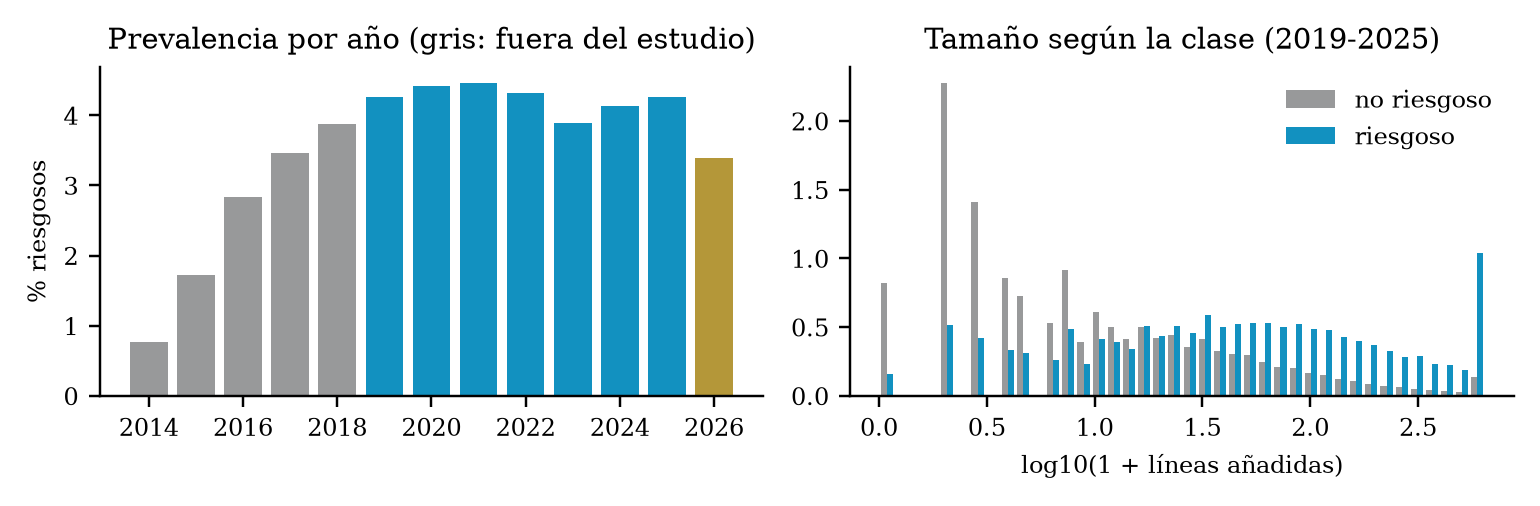
\includegraphics[width=\columnwidth]{../../resultados/e2/prevalencia_y_tamano.png}
\caption{Izquierda: prevalencia de commits riesgosos por año (en gris, los años fuera del estudio). Derecha: distribución del tamaño por clase en 2019--2025.}
\label{fig:eda}
\end{figure}

\subsection{Modelos y su papel}

La Tabla~\ref{tab:modelos} resume los modelos. Las dos referencias clásicas cubren dos extremos. La regresión logística es el estándar de JIT y es difícil de superar con partición temporal \cite{Kamei2013,Zeng2021}. El \emph{gradient boosting} \cite{Friedman2001} da la cota alta de una caja negra sobre las mismas variables.

\begin{table}[!t]
\caption{Modelos comparados}
\label{tab:modelos}
\centering\footnotesize
\begin{tabularx}{\columnwidth}{@{}l l Y@{}}
\toprule
\cabecera \textbf{Modelo} & \textbf{Papel} & \textbf{Justificación}\\
\midrule
Clase mayoritaria & Trivial & Su AUC-PR es la prevalencia: el piso\\
Reg.\ logística & Clásica & Estándar de JIT \cite{Kamei2013}; $\log(1+x)$ y estandarización\\
\emph{Gradient boosting} & Clásica fuerte & Cota alta sin restricción de interpretabilidad \cite{Friedman2001}\\
Difuso-evolutivo & Propuesto & $\le$15 reglas legibles; vértices y reglas ajustados con un AG\\
Difuso sin evolución & Variante de control & Mismas reglas iniciales, sin AG: mide el aporte de la evolución\\
\bottomrule
\end{tabularx}
\end{table}

\textbf{Qué propiedad de los datos aprovecha el modelo propuesto.} El riesgo crece por umbrales con el tamaño y la difusión, se modula con la revisión y la experiencia, y las variables tienen colas muy pesadas. Una partición difusa sobre la escala de cuantiles captura esos umbrales sin depender de la escala. Las reglas con pocos antecedentes capturan las interacciones que un mantenedor reconoce, por ejemplo ``si el cambio es grande y toca varios subsistemas''. El modelo usa 10 variables fijadas antes de ver resultados: líneas añadidas y borradas, archivos, subsistemas, \texttt{Reviewed-by}, \texttt{Signed-off-by}, si es corrección, si va a \emph{stable} y la experiencia del autor, en total y en el subsistema.

\subsection{Clasificador difuso-evolutivo}

Cada variable $x_j$ se lleva a $z_j\in[0,1]$ con su función de distribución empírica, estimada solo con el entrenamiento. Sobre $z_j$ se definen tres términos (bajo, medio, alto) que forman una partición de Ruspini \cite{Ruspini1969} con vértices $a_j<b_j<c_j$: bajo vale 1 hasta $a_j$ y cae a 0 en $b_j$; medio es el triángulo $(a_j,b_j,c_j)$; alto sube de 0 en $b_j$ a 1 en $c_j$. Una regla $r$ tiene hasta tres antecedentes y un peso $w_r\in[0,1]$:
\begin{equation}
\mu_r(\mathbf{x})=\prod_{(j,t)\in A_r}\mu_{jt}(z_j),\qquad
s(\mathbf{x})=1-\prod_{r}\bigl(1-w_r\,\mu_r(\mathbf{x})\bigr),
\end{equation}
es decir, t-norma producto y O probabilístico entre reglas. El puntaje $s$ ordena los commits por riesgo.

El ajuste sigue el enfoque Pittsburgh de los sistemas difusos genéticos \cite{Herrera2008,Ishibuchi2001}: cada individuo codifica todos los vértices y la base completa de reglas (activación, antecedentes, términos y pesos). La aptitud es el AUC-PR de entrenamiento, que es la métrica adecuada con clases desbalanceadas \cite{Saito2015}, menos una penalización por el número de antecedentes. Los operadores son:
\begin{itemize}
\item selección por torneo y elitismo;
\item cruce uniforme, que hereda cada regla completa;
\item mutación gaussiana de vértices y pesos, y mutación aleatoria de antecedentes y términos.
\end{itemize}

La variante sin evolución fija los vértices en los cuantiles $(0{,}2;\,0{,}5;\,0{,}8)$ y elige reglas de 1 o 2 antecedentes de forma voraz, por su confianza difusa, mientras mejore el AUC-PR. Esa misma solución siembra la población inicial del AG. Así, la diferencia entre ambas variantes aísla el aporte de la evolución.

\subsection{Pipeline sin fuga de información}

Todo lo que se aprende de los datos se ajusta solo con el entrenamiento de cada ventana y se aplica sin cambios a la validación o a la prueba:
\begin{itemize}
\item la transformación $\log(1+x)$ y la estandarización de la regresión logística, dentro de un \texttt{Pipeline};
\item la función de distribución empírica del modelo difuso;
\item el umbral de decisión.
\end{itemize}
No se balancean las clases: el AUC-PR se mide con la prevalencia real, y los conjuntos balanceados de forma artificial inflan el desempeño de manera engañosa \cite{Nguyen2025}. Las variables solo usan información anterior a la integración del commit. La experiencia del autor se cuenta con los commits previos en orden temporal.

\subsection{Partición temporal}

Nunca se mezclan commits al azar (Fig.~\ref{fig:particion}). Para cada año de validación $V\in\{2023,2024,2025\}$ se entrena con $[\text{2019-01-01},\ \text{inicio}(V)-90\text{ d})$ y se valida con el año $V$ completo. El hueco de 90 días replica lo que ocurre en la práctica: al entrenar, las etiquetas de los últimos 90 días todavía no existen. El modelo final se entrena con $[\text{2019-01-01},\ \text{2025-10-03})$ y se evalúa una sola vez con los \cifNPrueba{} commits de enero a julio de 2026 (prevalencia \cifPrevPrueba{}).

La partición de prueba quedó guardada con una huella SHA-256 de sus hashes y etiquetas. La evaluación final verifica de forma estricta que la huella no cambie. Se declara una salvedad: durante una fase preliminar de factibilidad, modelos simples se evaluaron una vez sobre 2026 para confirmar que había señal. Ninguna decisión posterior usó esas cifras.

\begin{figure}[!t]
\centering
% Partición temporal: ventana creciente con hueco de 90 días. Escala: 1 año = 0,85 cm desde 2019.
\begin{tikzpicture}[x=0.85cm,y=0.42cm,font=\scriptsize]
  \def\h{0.25}  % hueco de 90 días ~ 0,25 años
  \foreach \y/\lab/\ini in {3/V$_{2023}$/4, 2/V$_{2024}$/5, 1/V$_{2025}$/6}{
    \fill[udazul!70] (0,\y-0.32) rectangle (\ini-\h,\y+0.32);
    \fill[udplata!35] (\ini-\h,\y-0.32) rectangle (\ini,\y+0.32);
    \fill[uddorado!85] (\ini,\y-0.32) rectangle (\ini+1,\y+0.32);
    \node[left,udsable] at (0,\y) {\lab};
  }
  \fill[udazul!70] (0,-0.32) rectangle (7-\h,0.32);
  \fill[udplata!35] (7-\h,-0.32) rectangle (7,0.32);
  \fill[udrojo!80] (7,-0.32) rectangle (7+7/12,0.32);
  \node[left,udsable] at (0,0) {Prueba};
  \draw[udsable] (0,-0.75) -- (8,-0.75);
  \foreach \x/\t in {0/2019,1/2020,2/2021,3/2022,4/2023,5/2024,6/2025,7/2026}
    \draw[udsable] (\x,-0.75) -- ++(0,-0.12) node[below] {\t};
  \node[anchor=west,fill=udazul!70,minimum width=3mm,minimum height=2mm,inner sep=0] (a) at (0,4.2) {};
  \node[anchor=west] at (a.east) {entrenamiento};
  \node[anchor=west,fill=udplata!35,minimum width=3mm,minimum height=2mm,inner sep=0] (b) at (2.2,4.2) {};
  \node[anchor=west] at (b.east) {hueco 90 d};
  \node[anchor=west,fill=uddorado!85,minimum width=3mm,minimum height=2mm,inner sep=0] (c) at (4.1,4.2) {};
  \node[anchor=west] at (c.east) {validación};
  \node[anchor=west,fill=udrojo!80,minimum width=3mm,minimum height=2mm,inner sep=0] (d) at (5.9,4.2) {};
  \node[anchor=west] at (d.east) {prueba};
\end{tikzpicture}

\caption{Partición temporal con ventana creciente. Cada ventana de validación (2023, 2024 y 2025) se entrena con todo lo anterior menos un hueco de 90 días; la prueba (enero--julio de 2026) se evalúa una sola vez.}
\label{fig:particion}
\end{figure}

\subsection{Métricas y pruebas estadísticas}

\textbf{Métrica principal: AUC-PR} (precisión promedio de la clase riesgoso). Con una prevalencia cercana al 4\,\%, el AUC-ROC es engañosamente alto y el AUC-PR muestra la utilidad real de la lista de commits marcados \cite{Saito2015}. El AUC-PR de un clasificador sin información es igual a la prevalencia; por eso también se reporta el cociente AUC-PR/prevalencia.

\textbf{Métricas secundarias:} MCC, AUC-ROC, sensibilidad y especificidad. Las métricas que dependen de un umbral usan el que maximiza el MCC en la ventana de validación 2025, aplicado tal cual en la prueba.

\textbf{Costo:} tiempo de entrenamiento, tiempo de inferencia y número de parámetros.

\textbf{Incertidumbre.} Se reportan intervalos de confianza del 95\,\% por \emph{bootstrap} (1000 remuestreos de la prueba) y media $\pm$ desviación en 5 semillas (11, 23, 37, 41 y 53) para los modelos estocásticos.

\textbf{Pruebas.}
\begin{itemize}
\item McNemar con corrección de continuidad, entre el difuso-evolutivo y cada referencia, sobre las mismas predicciones de prueba \cite{Dietterich1998}.
\item Friedman con \emph{post hoc} de Nemenyi sobre los rangos de AUC-PR de los cinco modelos en las tres ventanas de validación más la prueba \cite{Demsar2006}.
\end{itemize}
En ambos casos $\alpha=0{,}05$. Con solo 5 semillas no se usa Wilcoxon. Una diferencia sin prueba se reporta como ``diferencia observada''.

\subsection{Resultados de validación de las referencias}

Las referencias se ajustaron con el mismo pipeline y la misma partición que el modelo propuesto. Se probó una pequeña rejilla y se eligió la configuración con mayor AUC-PR medio en las tres ventanas (Tabla~\ref{tab:referencias}).

\textbf{Mejor referencia clásica:} el \emph{gradient boosting}, con AUC-PR medio de \cifValGB{} y alrededor de \cifParamGB{} parámetros (nodos de los árboles). Es la referencia $R$ del criterio de éxito.

\textbf{Regresión logística:} da \cifValLogistica{} con \cifParamLR{} parámetros, y la regularización no cambia nada porque hay cientos de miles de ejemplos.

\textbf{Clase mayoritaria:} queda en \cifValMayoritaria{}, la prevalencia. Ambas referencias clásicas la multiplican por cerca de cuatro.

\begin{table*}[!t]
\caption{Validación de las referencias: AUC-PR por ventana, media y AUC-ROC medio (en negrita, la configuración elegida)}
\label{tab:referencias}
\centering\footnotesize
\begin{tabular}{@{}l l c c c c c@{}}
\toprule
\cabecera \textbf{Modelo} & \textbf{Configuración} & \textbf{2023} & \textbf{2024} & \textbf{2025} & \textbf{AUC-PR medio} & \textbf{AUC-ROC}\\
\midrule
\filas{../comun/tabla_referencias.tex}
\bottomrule
\end{tabular}
\end{table*}

\subsection{Espacio de hiperparámetros del modelo propuesto}

El espacio se declara antes de buscar (Tabla~\ref{tab:espacio}). La búsqueda es aleatoria, con 14 configuraciones de las 972 posibles. Cada configuración se evalúa en las tres ventanas con la semilla 11 y se elige por el AUC-PR medio. La sensibilidad se analiza sobre la rejilla de máximo de reglas $\times$ probabilidad de mutación, con el resto fijo en la mejor configuración. Después, la configuración elegida se entrena con las 5 semillas.

\begin{table}[!t]
\caption{Espacio de hiperparámetros del difuso-evolutivo}
\label{tab:espacio}
\centering\footnotesize
\begin{tabularx}{\columnwidth}{@{}l Y@{}}
\toprule
\cabecera \textbf{Hiperparámetro} & \textbf{Valores}\\
\midrule
\filas{../comun/tabla_espacio.tex}
\bottomrule
\end{tabularx}
\end{table}

%=====================================================================
\section{Experimentación}

Esta sección cubre el entrenamiento (fase F6). Todo se hizo sobre las ventanas de validación 2023--2025; la prueba de 2026 no interviene.

\subsection{Registro de experimentos}

El registro de experimentos guarda, de cada entrenamiento, la etapa, el modelo, la configuración, la semilla, la ventana, el tamaño de entrenamiento, el AUC-PR y el AUC-ROC de validación, el tiempo y el número de parámetros. Hay \cifRegReferencias{} corridas de las referencias y \cifRegPropuesto{} del modelo propuesto:
\begin{itemize}
\item \cifRegBusq{} de la búsqueda;
\item \cifRegSens{} de la sensibilidad;
\item 15 de las semillas;
\item 3 de la variante sin evolución.
\end{itemize}
Los entrenamientos corren en paralelo (6 procesos). Uno del difuso-evolutivo con la configuración final tarda unos \cifTiempoFE{} minutos con unos 450\,000 commits, porque la aptitud se evalúa sobre una muestra de 80\,000.

\subsection{Búsqueda aleatoria}

Se evaluaron \cifNBusqueda{} configuraciones del espacio de la Tabla~\ref{tab:espacio} en las tres ventanas (Tabla~\ref{tab:busqueda}). La mejor tiene la población y el número de generaciones más grandes del espacio y la mutación más baja, y alcanza un AUC-PR medio de \cifMejorBusqueda{}. Que gane el extremo del espacio sugiere que el AG aún tenía margen. No se amplió la búsqueda: se registra como limitación.

\begin{table*}[!t]
\caption{Búsqueda aleatoria: AUC-PR medio $\pm$ desviación en las tres ventanas de validación (semilla 11)}
\label{tab:busqueda}
\centering\footnotesize
\begin{tabular}{@{}c c c c c c c c@{}}
\toprule
\cabecera \textbf{Puesto} & \textbf{Máx.\ reglas} & \textbf{Población} & \textbf{Generaciones} & \textbf{Prob.\ mutación} & \textbf{Prob.\ cruce} & $\boldsymbol{\lambda}$ & \textbf{AUC-PR}\\
\midrule
\filas{../comun/tabla_busqueda.tex}
\bottomrule
\end{tabular}
\end{table*}

\subsection{Análisis de sensibilidad}

Con el resto fijo en la mejor configuración, se varió el máximo de reglas y la probabilidad de mutación (Fig.~\ref{fig:sensibilidad}).

\textbf{La mutación es lo que más pesa.} Con 0,05 el AUC-PR medio es \cifSensMutBaja{}; con 0,30 baja a \cifSensMutAlta{}. Una mutación alta destruye las reglas buenas antes de que se propaguen.

\textbf{El máximo de reglas casi no importa.} El mejor punto (\cifSensMaxR{} reglas, mutación \cifSensMaxPm{}) da \cifSensMax{}, prácticamente igual que con 5 o 15. El peor es \cifSensMinR{} reglas con mutación \cifSensMinPm{}, con \cifSensMin{}. Esto es coherente con lo que el AG hace en la práctica: aunque se le permitan 15 reglas, termina usando entre \cifReglasMin{} y \cifReglasMax{}.

La configuración congelada es la de la búsqueda (15 reglas como máximo). No se cambió a 10 después de ver la sensibilidad, porque la diferencia (0,001) está dentro de la variación entre semillas.

\begin{figure}[!t]
\centering
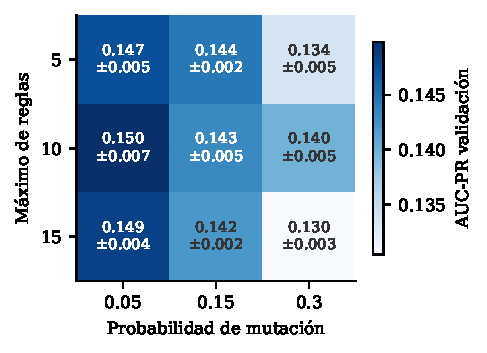
\includegraphics[width=0.82\columnwidth]{../../resultados/figuras/sensibilidad.pdf}
\caption{Sensibilidad: AUC-PR medio $\pm$ desviación en las tres ventanas, según el máximo de reglas y la probabilidad de mutación.}
\label{fig:sensibilidad}
\end{figure}

\subsection{Convergencia}

La Fig.~\ref{fig:convergencia} muestra la aptitud del mejor individuo y la mediana de la población, por generación, en la ventana 2025 para las 5 semillas. La mejora es rápida en las primeras 20 generaciones y se estabiliza entre la 60 y la 80. La distancia entre el mejor individuo y la mediana se mantiene, así que la población conserva diversidad hasta el final.

\begin{figure}[!t]
\centering
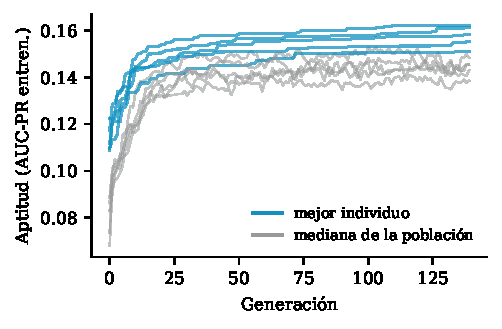
\includegraphics[width=0.92\columnwidth]{../../resultados/figuras/curva_aprendizaje.pdf}
\caption{Curva de aprendizaje del AG (ventana 2025, 5 semillas): aptitud del mejor individuo y mediana de la población.}
\label{fig:convergencia}
\end{figure}

\subsection{Semillas y aporte de la evolución}

La configuración elegida se entrenó con las 5 semillas (Tabla~\ref{tab:semillas}). El AUC-PR medio de validación es \cifValFE{} $\pm$ \cifValFEde{}. Es la diferencia observada respecto a las referencias, sin prueba de significancia todavía:
\begin{itemize}
\item prácticamente igual a la regresión logística (\cifValLogistica{});
\item el \cifRazonValFE{} del \emph{gradient boosting} (\cifValGB{});
\item muy por encima de la prevalencia.
\end{itemize}

La variante sin evolución arranca de la misma solución voraz y se queda en \cifValVariante{}. Usa \cifReglasVariante{} reglas con \cifAntVariante{} antecedentes. El AG no solo mejora el AUC-PR: también simplifica el modelo a entre \cifReglasMin{} y \cifReglasMax{} reglas, con \cifAntMin{} a \cifAntMax{} antecedentes en total.

\begin{table*}[!t]
\caption{Difuso-evolutivo con 5 semillas y variante sin evolución (validación)}
\label{tab:semillas}
\centering\footnotesize
\begin{tabular}{@{}l c c c c c c c@{}}
\toprule
\cabecera \textbf{Semilla} & \textbf{2023} & \textbf{2024} & \textbf{2025} & \textbf{Media} & \textbf{Reglas} & \textbf{Antec.} & \textbf{Tiempo (s)}\\
\midrule
\filas{../comun/tabla_semillas.tex}
\bottomrule
\end{tabular}
\end{table*}

\subsection{Configuración congelada}

Se congeló la configuración final antes de evaluar la prueba. Contiene:
\begin{itemize}
\item los hiperparámetros del difuso-evolutivo y las 5 semillas;
\item el umbral de MCC de cada semilla en la ventana 2025;
\item la semilla de referencia para McNemar (\cifSemillaRef{}, la de AUC-PR mediano);
\item la configuración y el umbral de cada referencia, con $R$ = \emph{gradient boosting};
\item la huella SHA-256 de la partición de prueba (\texttt{\cifHuella}\ldots).
\end{itemize}
El modelo final se entrena con todo 2019 hasta el 3 de octubre de 2025 y se evalúa una sola vez en 2026.


%=====================================================================
\section*{Declaración de uso de IA generativa}
{\footnotesize Usé Gemini para revisar y corregir errores y para redactar este informe a partir de los resultados del cuaderno y la recuperación de algunos papers para la evaluación del mismo.}


% Generado por revision/generar_e1.py 4 en orden de cita; no editar a mano.
\begin{thebibliography}{44}
\bibitem{Mockus2000} A. Mockus and D. M. Weiss, ``Predicting risk of software changes,'' Bell Labs Tech. J., vol. 5, no. 2, pp. 169--180, Apr.--Jun. 2000, doi: \mbox{10.1002/bltj.2229}.
\bibitem{Kamei2013} Y. Kamei, E. Shihab, B. Adams, A. E. Hassan, A. Mockus, A. Sinha, and N. Ubayashi, ``A large-scale empirical study of just-in-time quality assurance,'' IEEE Trans. Softw. Eng., vol. 39, no. 6, pp. 757--773, Jun. 2013, doi: \mbox{10.1109/TSE.2012.70}.
\bibitem{Sliwerski2005} J. Śliwerski, T. Zimmermann, and A. Zeller, ``When do changes induce fixes?'' in Proc. Int. Workshop Mining Softw. Repositories (MSR '05), St. Louis, MO, USA, 2005, pp. 1--5, doi: \mbox{10.1145/1083142.1083147}.
\bibitem{Lyu2024} Y. Lyu, H. J. Kang, R. Widyasari, J. Lawall, and D. Lo, ``Evaluating SZZ implementations: An empirical study on the Linux kernel,'' IEEE Trans. Softw. Eng., vol. 50, no. 9, pp. 2219--2239, Sep. 2024, doi: \mbox{10.1109/TSE.2024.3406718}.
\bibitem{KernelAdd} S. Levin, ``docs: add AI Coding Assistants documentation,'' Linux kernel, commit 78d979db6cef, Jan. 6, 2026. [Online]. Available: \url{https://github.com/torvalds/linux/commit/78d979db6cef}
\bibitem{KernelSimpl} C. Brauner, ``coding-assistants: simplify attribution,'' Linux kernel, commit 816d9992d9ed, Aug. 3, 2026. [Online]. Available: \url{https://github.com/torvalds/linux/commit/816d9992d9ed}
\bibitem{KernelRemove} S. Levin, ``docs: remove Assisted-by references,'' Linux kernel, commit 1e035297ffda, Oct. 14, 2026. [Online]. Available: \url{https://github.com/torvalds/linux/commit/1e035297ffda}
\bibitem{Studer2021} S. Studer, T. B. Bui, C. Drescher, A. Hanuschkin, L. Winkler, S. Peters, and K.-R. M\"uller, ``Towards CRISP-ML(Q): A machine learning process model with quality assurance methodology,'' Mach. Learn. Knowl. Extr., vol. 3, no. 2, pp. 392--413, 2021, doi: 10.3390/make3020020.
\bibitem{MaesBermejo2024} M. Maes Bermejo, J. M. González-Barahona, M. Gallego, and G. Robles, ``A dataset of Linux kernel commits'' (v3), Zenodo, 2024, doi: 10.5281/zenodo.10654193.
\bibitem{Page2021} M. J. Page \emph{et al.}, ``The PRISMA 2020 statement: An updated guideline for reporting systematic reviews,'' BMJ, vol. 372, Art. no. n71, 2021, doi: 10.1136/bmj.n71.
\bibitem{Zeng2021} Z. Zeng, Y. Zhang, H. Zhang, and L. Zhang, ``Deep just-in-time defect prediction: How far are we?'' in Proc. 30th ACM SIGSOFT Int. Symp. Softw. Testing Anal. (ISSTA), Virtual, Denmark, 2021, pp. 427--438, doi: \mbox{10.1145/3460319.3464819}.
\bibitem{Ni2022} C. Ni, W. Wang, K. Yang, X. Xia, K. Liu, and D. Lo, ``The best of both worlds: Integrating semantic features with expert features for defect prediction and localization,'' in Proc. 30th ACM Joint Eur. Softw. Eng. Conf. Symp. Found. Softw. Eng. (ESEC/FSE), Singapore, 2022, pp. 672--683, doi: \mbox{10.1145/3540250.3549165}.
\bibitem{Liu2026} Y. Liu, K. Jabre, R. Abreu, Z. J. Carmichael, V. Murali, A. Patel, J. Ge, W. Sun, C. Zhang, A. Mockus, D. Khavari, P. C. Rigby, and N. Nagappan, ``A preliminary study on explaining risk of code changes using LLM-based prediction models,'' in Proc. 3rd ACM Int. Conf. AI-Powered Softw. (AIware '26), Montreal, QC, Canada, 2026, pp. 259--267, doi: \mbox{10.1145/3805760.3814916}.
\bibitem{JITLine2021} C. Pornprasit and C. K. Tantithamthavorn, ``JITLine: A simpler, better, faster, finer-grained just-in-time defect prediction,'' in Proc. IEEE/ACM 18th Int. Conf. Mining Softw. Repositories (MSR), 2021, pp. 369--379, doi: \mbox{10.1109/MSR52588.2021.00049}.
\bibitem{PyExplainer2021} C. Pornprasit, C. Tantithamthavorn, J. Jiarpakdee, M. Fu, and P. Thongtanunam, ``PyExplainer: Explaining the predictions of just-in-time defect models,'' in Proc. 36th IEEE/ACM Int. Conf. Automated Softw. Eng. (ASE), 2021, pp. 407--418, doi: \mbox{10.1109/ASE51524.2021.9678763}.
\bibitem{Aftab2023} S. Aftab, S. Abbas, T. M. Ghazal, M. Ahmad, H. A. Hamadi, C. Y. Yeun, and M. A. Khan, ``A cloud-based software defect prediction system using data and decision-level machine learning fusion,'' Mathematics, vol. 11, no. 3, Art. no. 632, 2023, doi: \mbox{10.3390/math11030632}.
\bibitem{Dey2025} R. Dey, J. Piri, B. Acharya, P. P. Das, V. C. Gerogiannis, and A. Kanavos, ``A hybrid evolutionary fuzzy ensemble approach for accurate software defect prediction,'' Mathematics, vol. 13, no. 7, Art. no. 1140, 2025, doi: \mbox{10.3390/math13071140}.
\bibitem{McIntosh2018} S. McIntosh and Y. Kamei, ``Are fix-inducing changes a moving target? A longitudinal case study of just-in-time defect prediction,'' IEEE Trans. Softw. Eng., vol. 44, no. 5, pp. 412--428, May 2018, doi: \mbox{10.1109/TSE.2017.2693980}.
\bibitem{Cabral2019} G. G. Cabral, L. L. Minku, E. Shihab, and S. Mujahid, ``Class imbalance evolution and verification latency in just-in-time software defect prediction,'' in Proc. IEEE/ACM 41st Int. Conf. Softw. Eng. (ICSE), Montreal, QC, Canada, 2019, pp. 666--676, doi: \mbox{10.1109/ICSE.2019.00076}.
\bibitem{Olewicki2024} D. Olewicki, S. Habchi, M. Nayrolles, M. Faramarzi, S. Chandar, and B. Adams, ``On the costs and benefits of adopting lifelong learning for software analytics -- Empirical study on brown build and risk prediction,'' in Proc. 46th Int. Conf. Softw. Eng.: Softw. Eng. Pract. (ICSE-SEIP), Lisbon, Portugal, 2024, pp. 275--286, doi: \mbox{10.1145/3639477.3639717}.
\bibitem{Nguyen2025} D. Nguyen, T. Le-Cong, T. H. M. Le, M. A. Babar, and Q.-T. Huynh, ``Toward realistic evaluations of just-in-time vulnerability prediction,'' in Proc. IEEE Int. Conf. Softw. Maint. Evol. (ICSME), Auckland, New Zealand, 2025, pp. 1--10, doi: \mbox{10.1109/ICSME64153.2025.00023}.
\bibitem{Mazloomzadeh2026} I. Mazloomzadeh, M. M. Morovati, and F. Khomh, ``How do AI coding agents contribute to software development? An empirical study of agentic pull requests,'' arXiv:2607.21832, Jul. 2026, doi: \mbox{10.48550/arXiv.2607.21832}.
\bibitem{Herbold2022} S. Herbold, A. Trautsch, F. Trautsch, and B. Ledel, ``Problems with SZZ and features: An empirical study of the state of practice of defect prediction data collection,'' Empir. Softw. Eng., vol. 27, no. 2, Art. no. 42, 2022, doi: \mbox{10.1007/s10664-021-10092-4}.
\bibitem{Falessi2022} D. Falessi, A. Ahluwalia, and M. Di Penta, ``The impact of dormant defects on defect prediction: A study of 19 Apache projects,'' ACM Trans. Softw. Eng. Methodol., vol. 31, no. 1, pp. 1--26, Jan. 2022, doi: \mbox{10.1145/3467895}.
\bibitem{Jiarpakdee2021} J. Jiarpakdee, C. K. Tantithamthavorn, and J. Grundy, ``Practitioners' perceptions of the goals and visual explanations of defect prediction models,'' in Proc. IEEE/ACM 18th Int. Conf. Mining Softw. Repositories (MSR), 2021, pp. 432--443, doi: \mbox{10.1109/MSR52588.2021.00055}.
\bibitem{Sahar2024} H. Sahar, A. A. Bangash, A. Hindle, and D. Barbosa, ``IRJIT: A simple, online, information retrieval approach for just-in-time software defect prediction,'' Empir. Softw. Eng., vol. 29, no. 5, Art. no. 131, 2024, doi: \mbox{10.1007/s10664-024-10514-z}.
\bibitem{Yu2024FoX} J. Yu, M. Fu, A. Ignatiev, C. Tantithamthavorn, and P. Stuckey, ``A formal explainer for just-in-time defect predictions,'' ACM Trans. Softw. Eng. Methodol., vol. 33, no. 7, pp. 1--31, Sep. 2024, doi: \mbox{10.1145/3664809}.
\bibitem{Chen2018MULTI} X. Chen, Y. Zhao, Q. Wang, and Z. Yuan, ``MULTI: Multi-objective effort-aware just-in-time software defect prediction,'' Inf. Softw. Technol., vol. 93, pp. 1--13, Jan. 2018, doi: \mbox{10.1016/j.infsof.2017.08.004}.
\bibitem{Kang2021} J. Kang, S. Kwon, D. Ryu, and J. Baik, ``HASPO: Harmony search-based parameter optimization for just-in-time software defect prediction in maritime software,'' Appl. Sci., vol. 11, no. 5, Art. no. 2002, 2021, doi: \mbox{10.3390/app11052002}.
\bibitem{Mostafa2025} S. Mostafa, S. T. Cynthia, B. Roy, and D. Mondal, ``Feature transformation for improved software bug detection and commit classification,'' J. Syst. Softw., vol. 219, Art. no. 112205, Jan. 2025, doi: \mbox{10.1016/j.jss.2024.112205}.
\bibitem{Chen2025} F. Chen, Y. Ke, X. Liu, and Q. Wei, ``Multi-project just-in-time software defect prediction based on multi-task learning for mobile applications,'' in Proc. IEEE Conf. Softw. Testing, Verification Validation (ICST), 2025, pp. 127--137, doi: \mbox{10.1109/ICST62969.2025.10989004}.
\bibitem{Shehab2023} M. A. Shehab, A. Hamou-Lhadj, and V. S. P. Gunda, ``JITBoost: Boosting just-in-time defect prediction using Boolean combination of classifiers,'' in Proc. IEEE 23rd Int. Conf. Softw. Qual., Rel. Secur. (QRS), 2023, pp. 95--104, doi: \mbox{10.1109/QRS60937.2023.00019}.
\bibitem{Chitsazian2026} Z. Chitsazian, S. Sedighian Kashi, and A. Nikanjam, ``Detecting concept drift in just-in-time software defect prediction using model interpretation,'' Int. J. Syst. Assur. Eng. Manag., vol. 17, no. 9, pp. 2701--2722, 2026, doi: \mbox{10.1007/s13198-025-03122-7}.
\bibitem{Patel2024} H. J. Patel, B. Adams, and A. E. Hassan, ``Post deployment recycling of machine learning models,'' Empir. Softw. Eng., vol. 29, no. 4, Art. no. 100, 2024, doi: \mbox{10.1007/s10664-024-10492-2}.
\bibitem{Tian2026} D. Tian, L. Song, and X. Su, ``Just-in-time quality assurance with assistance of automated defect prediction and code testing,'' ACM Trans. Softw. Eng. Methodol., vol. 35, no. 9, pp. 1--46, 2026, doi: \mbox{10.1145/3779653}.
\bibitem{Song2023} L. Song and L. L. Minku, ``A procedure to continuously evaluate predictive performance of just-in-time software defect prediction models during software development,'' IEEE Trans. Softw. Eng., vol. 49, no. 2, pp. 646--666, Feb. 2023, doi: \mbox{10.1109/TSE.2022.3158831}.
\bibitem{Veras2025} R. C. Veras, G. G. Cabral, and A. L. I. de Oliveira, ``Semantic SZZ: Mitigating the impact of misclassified corrective changes in just-in-time software defect prediction,'' in Proc. IEEE Int. Conf. Syst., Man, Cybern. (SMC), 2025, pp. 769--774, doi: \mbox{10.1109/SMC58881.2025.11342537}.
\bibitem{Friedman2001} J. H. Friedman, ``Greedy function approximation: A gradient boosting machine,'' Ann. Statist., vol. 29, no. 5, pp. 1189--1232, Oct. 2001, doi: \mbox{10.1214/aos/1013203451}.
\bibitem{Ruspini1969} E. H. Ruspini, ``A new approach to clustering,'' Inf. Control, vol. 15, no. 1, pp. 22--32, Jul. 1969, doi: \mbox{10.1016/S0019-9958(69)90591-9}.
\bibitem{Herrera2008} F. Herrera, ``Genetic fuzzy systems: taxonomy, current research trends and prospects,'' Evol. Intell., vol. 1, no. 1, pp. 27--46, Mar. 2008, doi: \mbox{10.1007/s12065-007-0001-5}.
\bibitem{Ishibuchi2001} H. Ishibuchi, T. Nakashima, and T. Murata, ``Three-objective genetics-based machine learning for linguistic rule extraction,'' Inf. Sci., vol. 136, no. 1--4, pp. 109--133, Aug. 2001, doi: \mbox{10.1016/S0020-0255(01)00144-X}.
\bibitem{Saito2015} T. Saito and M. Rehmsmeier, ``The precision-recall plot is more informative than the ROC plot when evaluating binary classifiers on imbalanced datasets,'' PLOS ONE, vol. 10, no. 3, Art. no. e0118432, Mar. 2015, doi: \mbox{10.1371/journal.pone.0118432}.
\bibitem{Dietterich1998} T. G. Dietterich, ``Approximate statistical tests for comparing supervised classification learning algorithms,'' Neural Comput., vol. 10, no. 7, pp. 1895--1923, Oct. 1998, doi: \mbox{10.1162/089976698300017197}.
\bibitem{Demsar2006} J. Demšar, ``Statistical comparisons of classifiers over multiple data sets,'' J. Mach. Learn. Res., vol. 7, pp. 1--30, 2006. [Online]. Available: \url{https://jmlr.org/papers/v7/demsar06a.html}
\end{thebibliography}


\end{document}
